% ============================================================
% 第三章 第3.2节：状态依赖自适应协同（SDAS）模型的
%              软件实现
% 独立编译包装
% ============================================================
\documentclass[12pt,a4paper]{report}

% ---- 中文支持 ----
\usepackage{fontspec}
\usepackage{xeCJK}
\setCJKmainfont{SimSun}
\setCJKsansfont{SimHei}
\setCJKmonofont{FangSong}

% ---- 数学公式 ----
\usepackage{amsmath,amssymb}
\usepackage{bm}

% ---- 代码片段 ----
\usepackage{listings}
\lstset{
    basicstyle=\ttfamily\small,
    numbers=left,
    numberstyle=\tiny,
    frame=single,
    breaklines=true,
    language=Python,
    captionpos=b,
    tabsize=4,
    showstringspaces=false,
}

% ---- 算法环境 ----
\usepackage{algorithm}
\usepackage{algpseudocode}



% ---- 图片 ----
\usepackage{graphicx}
\usepackage{caption}
\usepackage{subcaption}
\graphicspath{{./figures/}}

% ---- 表格 ----
\usepackage{booktabs}
\usepackage{array}
\usepackage{multirow}

% ---- 引用与交叉引用 ----
\usepackage[colorlinks=true, linkcolor=black, citecolor=black]{hyperref}

% ---- 页面设置 ----
\usepackage{geometry}
\geometry{left=2.5cm,right=2.5cm,top=2.5cm,bottom=2.5cm}
\usepackage{setspace}
\linespread{1.3}

% ---- 符号宏 ----
\newcommand{\R}{\mathbb{R}}
\newcommand{\E}{\mathbf{E}}
\newcommand{\q}{\mathbf{q}}
\newcommand{\T}{\mathsf{T}}

\begin{document}

\setcounter{section}{3}
\setcounter{subsection}{1}

% ============================================================
% 第三章 第3.2节：状态依赖自适应协同（SDAS）模型的
%              软件实现
% ============================================================

\subsection{状态依赖自适应协同（SDAS）模型的软件实现}
\label{sec:sdas_implementation}

本节基于第\,\ref{sec:sdas_theory} 节建立的 SDAS 理论框架，系统地介绍该模型在 Python 编程环境中的完整软件实现。在进入具体实现细节之前，本节首先概述软件系统的整体架构与数据流。

\subsubsection{软件架构与数据流}
\label{sec:architecture}

本文开发的折纸手仿真工具包 \verb|synergy_hand_sim| 在功能上涵盖从 CAD 设计到交互式三维物理仿真的完整流程。就 SDAS 模型而言，其核心计算链路由以下六个功能层次组成：

\begin{enumerate}
    \item \textbf{设计层（CAD 编辑器模块）}：\verb|src/origami_cad/| 包基于 PyQt5 实现了图形化的折纸手设计编辑器。用户通过该编辑器在二维画布上绘制折痕线（区分峰折/谷折/轮廓）、添加面片、放置滑轮和孔类导向元件、定义缆绳路径与驱动器属性。编辑器内置了面片拓扑自动重建和设计验证功能。完成设计后，用户可将所有几何与拓扑信息保存为 \verb|.ohd| 文件（JSON 格式），该文件是连接设计与仿真的桥梁。
    \item \textbf{数据模型层}：以 \verb|OrigamiHandDesign| 类为核心容器，管理折痕线（\verb|fold_lines|）、面片（\verb|faces|）、滑轮（\verb|pulleys|）、孔（\verb|holes|）、腱绳路径（\verb|tendons|）和驱动器（\verb|actuators|）等全部设计数据。该层仅负责存储和查询，不涉及任何算法逻辑。
    \item \textbf{传动计算层}：\verb|TransmissionBuilder| 模块实现 \verb|compute_R_one_sided()| 函数，从 \verb|OrigamiHandDesign| 中提取单侧 Capstan 衰减传动向量 $\mathbf{R}_A$ 和 $\mathbf{R}_B$。
    \item \textbf{协同求解层}：\verb|SDASModel| 类封装了第\,\ref{sec:sdas_theory} 节中的 Schur 补公式和单向公式。在构造阶段接收传动向量 $\mathbf{R}_A$ 和 $\mathbf{R}_B$，预计算所有系数矩阵；在运行阶段接收电机位移输入，输出满足传动约束的关节角度向量。
    \item \textbf{仿真层}：包含两套并行的仿真机制。\textbf{运动学交互仿真器}（\verb|MuJoCoSimulator|）基于 MuJoCo 物理引擎，通过滑块回调接口实时驱动三维模型；\textbf{动力学数值仿真器}（\verb|HandSimulator|）包含惯性与阻尼模型，通过 ODE 积分输出关节角度的时间历程。
    \item \textbf{可视化层}：MuJoCo 原生 GLFW 查看器提供三维渲染，滑块面板提供交互控制；动力学仿真和运动学仿真的结果还可通过 MeshCat 浏览器端可视化或 \verb|SimulationVisualizer| 生成多面板图表。
\end{enumerate}

图\,\ref{fig:architecture} 展示了上述模块之间完整的数据流关系。系统以 Origami CAD 编辑器为设计入口，所有几何和拓扑信息通过 \verb|.ohd| 文件传递至数据模型层，随后分流至 URDF 导出和传动矩阵计算两条路径，最终汇聚于 MuJoCo 交互式仿真器和动力学数值仿真器。

\begin{figure}[htbp]
    \centering
    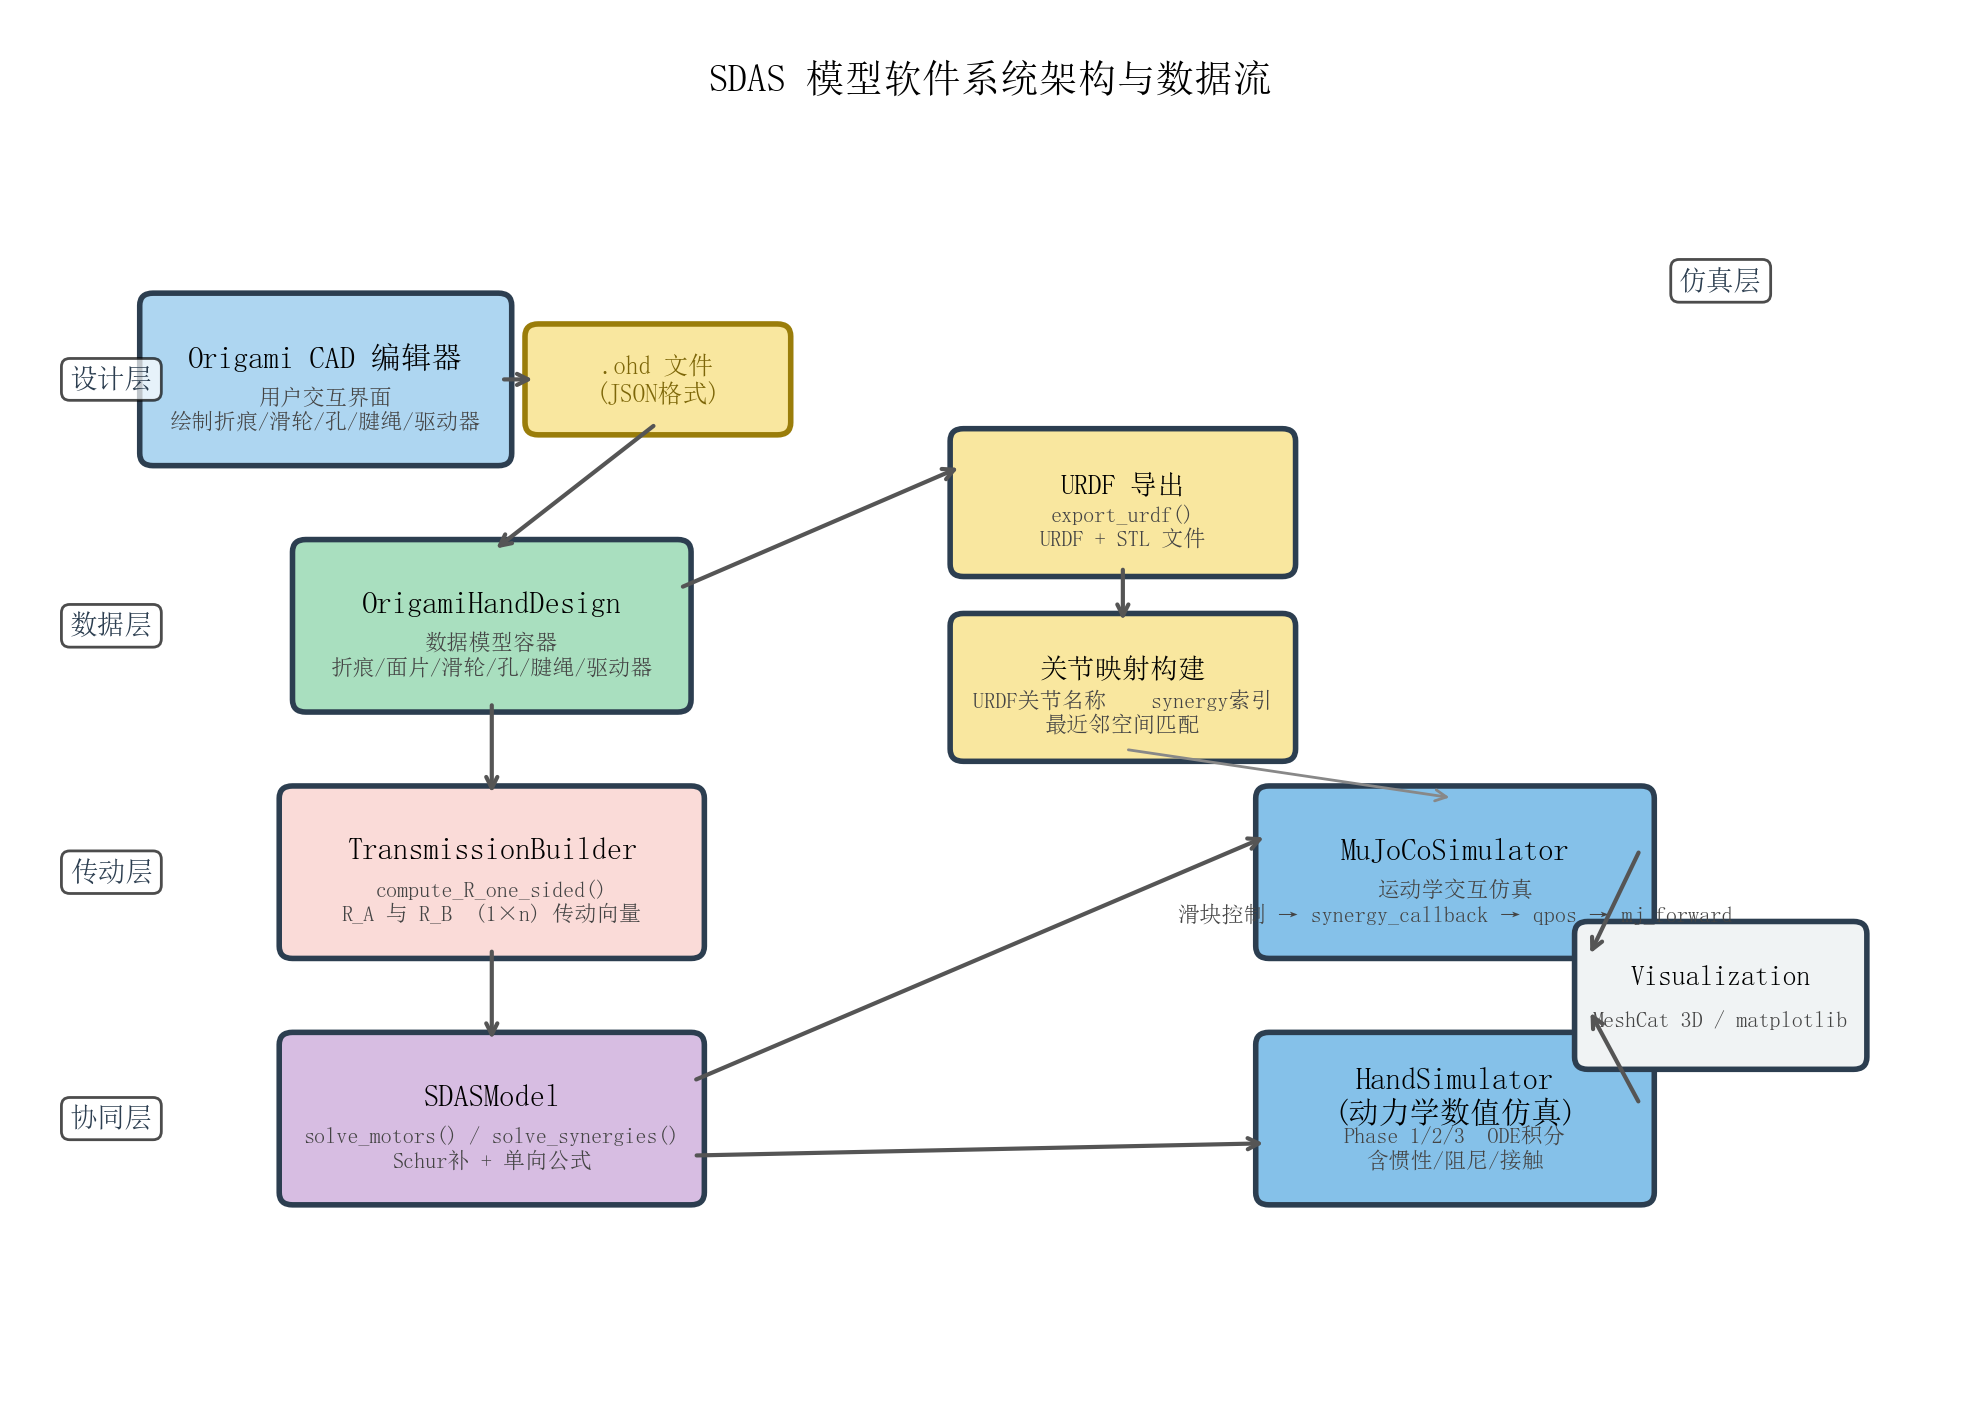
\includegraphics[width=0.92\textwidth]{figures/architecture_diagram.png}
    \caption{SDAS 模型软件系统架构与数据流。方框代表功能模块，箭头表示数据流向。左侧纵向排列了从设计层到协同层的四层结构，右侧为仿真层与可视化层。}
    \label{fig:architecture}
\end{figure}

以下 Python 脚本可生成图\,\ref{fig:architecture} 所示的系统架构图。该脚本基于 \verb|matplotlib| 库，通过 \verb|FancyBboxPatch| 绘制圆角矩形模块，使用 \verb|annotate| 绘制带箭头的连线标注数据流。运行时生成 \verb|architecture_diagram.png| 文件。

\begin{lstlisting}[language=Python, caption=系统架构图生成脚本]
import matplotlib.pyplot as plt
import matplotlib.patches as mpatches

def draw_box(ax, center, width, height, text, subtext='',
             facecolor='#D6EAF8', edgecolor='#2C3E50'):
    x, y = center
    rect = mpatches.FancyBboxPatch(
        (x - width/2, y - height/2), width, height,
        boxstyle="round,pad=0.1",
        facecolor=facecolor, edgecolor=edgecolor, lw=2)
    ax.add_patch(rect)
    ax.text(x, y + height*0.15, text, ha='center', va='center',
            fontsize=10, fontweight='bold')
    if subtext:
        ax.text(x, y - height*0.20, subtext, ha='center', va='center',
                fontsize=8, color='#444444')

def draw_io_box(ax, center, width, height, text,
                facecolor='#F9E79F', edgecolor='#9A7D0A'):
    x, y = center
    rect = mpatches.FancyBboxPatch(
        (x - width/2, y - height/2), width, height,
        boxstyle="round,pad=0.1",
        facecolor=facecolor, edgecolor=edgecolor, lw=2)
    ax.add_patch(rect)
    ax.text(x, y, text, ha='center', va='center',
            fontsize=9, fontweight='bold', color='#7D6608')

fig, ax = plt.subplots(figsize=(12, 8))
ax.set_xlim(-1, 13); ax.set_ylim(-1, 9); ax.axis('off')
draw_box(ax, (1.0, 7.0), 2.6, 1.2, 'Origami CAD Editor',
         'User interface\nfolds/pulleys/holes/tendon paths',
         facecolor='#AED6F1')
draw_io_box(ax, (3.5, 7.0), 1.8, 0.7, '.ohd File\n(JSON)')
draw_box(ax, (2.25, 5.0), 2.8, 1.2, 'OrigamiHandDesign',
         'Data container\nfolds/faces/pulleys/tendons',
         facecolor='#A9DFBF')
draw_box(ax, (2.25, 3.0), 3.0, 1.2, 'TransmissionBuilder',
         'compute_R_one_sided()\nR_A, R_B vectors',
         facecolor='#FADBD8')
draw_box(ax, (2.25, 1.0), 3.0, 1.2, 'SDASModel',
         'solve_motors() / solve_synergies()\nSchur complement',
         facecolor='#D7BDE2')
draw_box(ax, (7.0, 6.0), 2.4, 1.0, 'URDF Export',
         'export_urdf()\nURDF + STL files',
         facecolor='#F9E79F')
draw_box(ax, (7.0, 4.5), 2.4, 1.0, 'Joint Mapping',
         'URDF joint name to\nsynergy index mapping',
         facecolor='#F9E79F')
draw_box(ax, (9.5, 3.0), 2.8, 1.2, 'MuJoCoSimulator',
         'Interactive simulation\nslider control',
         facecolor='#85C1E9')
draw_box(ax, (9.5, 1.0), 2.8, 1.2, 'HandSimulator',
         'Numerical dynamics\nODE integration',
         facecolor='#85C1E9')
draw_box(ax, (11.5, 2.0), 2.0, 1.0, 'Visualization',
         'MeshCat / matplotlib',
         facecolor='#F0F3F4')
# Connect boxes with arrows (annotate)
for (sx, sy), (ex, ey) in [
    ((2.3, 7.0), (2.6, 7.0)),   # CAD -> .ohd
    ((3.5, 6.65), (3.5, 5.6)),  # .ohd -> OrigamiHandDesign
    ((3.65, 5.3), (5.8, 6.0)),  # OrigamiHandDesign -> URDF
    ((2.25, 4.4), (2.25, 3.6)), # OrigamiHandDesign -> TransmissionBuilder
    ((2.25, 2.4), (2.25, 1.6)), # TransmissionBuilder -> SDAS
    ((7.0, 5.5), (7.0, 5.0)),   # URDF -> Joint Mapping
    ((3.75, 1.3), (8.1, 3.3)),  # SDAS -> MuJoCo
    ((3.75, 0.7), (8.1, 1.2)),  # SDAS -> HandSimulator
    ((10.9, 3.3), (10.5, 2.5)), # MuJoCo -> Visualization
    ((10.9, 1.3), (10.5, 2.0)), # HandSimulator -> Visualization
]:
    ax.annotate('', xy=(ex, ey), xytext=(sx, sy),
                arrowprops=dict(arrowstyle='->', color='#555555', lw=1.5))
plt.title('SDAS Software System Architecture', fontsize=14, fontweight='bold')
plt.savefig('architecture_diagram.png', dpi=200, bbox_inches='tight')
\end{lstlisting}

运行该脚本即可生成图\,\ref{fig:architecture} 所示的系统架构图。

\subsubsection{核心数据结构：OrigamiHandDesign}
\label{sec:data_structures}

SDAS 模型软件实现的数据基础是 \verb|OrigamiHandDesign| 类（见 \verb|src/models/origami_design.py|）。该类的设计遵循``数据与算法分离''原则——类本身仅负责存储和查询，不涉及传动矩阵计算或运动学求解等算法逻辑。与 SDAS 模型密切相关的成员字段及其含义列于表\,\ref{tab:design_fields}。

\begin{table}[htbp]
\centering
\caption{\texttt{OrigamiHandDesign} 中与 SDAS 模型密切相关的关键属性}
\label{tab:design_fields}
\small
\begin{tabular}{@{}p{2.6cm}p{2.8cm}p{8.0cm}@{}}
\toprule
\textbf{字段} & \textbf{数据类型} & \textbf{说明} \\
\midrule
\verb|fold_lines| & \verb|dict[int, FoldLine]| & 所有折痕线字典。每个 \verb|FoldLine| 包含起止点坐标、折痕类型
（MOUNTAIN/VALLEY/OUTLINE）和弯曲刚度系数 $\kappa_i$。每个活动关节对应一条折痕线。\\
\verb|faces| & \verb|dict[int, OrigamiFace]| & 面片字典。每个面片由顶点序列和边 ID 序列定义，用于 URDF 导出和碰撞检测网格生成。\\
\verb|joints| & \verb|list[JointConnection]| & 关节连接表。每条记录包含关联的折痕线 ID、两个面片 ID 和折痕类型，描述相邻面片间的转动自由度。\\
\verb|pulleys| & \verb|dict[int, Pulley]| & 滑轮字典。滑轮 ID 为正整数，包含位置、半径 $r$、摩擦系数 $\mu$ 和附着折痕 ID。\\
\verb|holes| & \verb|dict[int, Hole]| & 孔字典。孔 ID $\le -100$，包含位置、板厚偏移 $h$、摩擦系数 $\mu$ 和附着折痕 ID。\\
\verb|tendons| & \verb|dict[int, Tendon]| & 腱绳路径字典。记录元素 ID 序列：正数为滑轮，$-1$ 为驱动器 A，$-2$ 为驱动器 B，$\le -100$ 为孔，$\le -200$ 为阻尼器。\\
\verb|actuators| & \verb|dict[int, Actuator]| & 驱动器字典。预定义两个驱动器，ID 分别为 $-1$（Motor A）和 $-2$（Motor B）。\\
\verb|dampers| & \verb|dict[int, Damper]| & 阻尼器字典。用于动态协同模型，SDAS 模型不使用该字段。\\
\bottomrule
\end{tabular}
\end{table}

关节索引的获取通过 \verb|get_joint_list()| 函数完成。该函数位于 \verb|src/models/transmission_builder.py|，其返回值包含两个元素：按 ID 排序的 \verb|JointConnection| 列表，以及 \verb|fold_line_id| 到关节索引的映射字典。当设计尚未重建拓扑时，函数直接从 \verb|fold_lines| 中筛选谷折和山折类型的折痕线作为关节，从而保留原始的 \verb|fold_line_ID|，使滑轮和孔中记录的 \verb|attached_fold_line_id| 与关节索引之间的映射关系不断裂。

从 SDAS 模型的角度来看，腱绳路径的拓扑结构是最关键的信息。以表\,\ref{tab:design_fields} 中的 \verb|tendons| 字段为例，一条包含元素序列 $[e_0, e_1, \ldots, e_{N-1}]$ 的腱绳中，$e_0 = -1$（Motor A）、$e_{N-1} = -2$（Motor B），中间元素为滑轮或孔。该序列唯一确定了从两台驱动器出发的 Capstan 张力衰减路径，从而决定了 $\mathbf{R}_A$ 与 $\mathbf{R}_B$ 两个传动向量的分布。\verb|tendons| 中的元素 ID 编码约定由 CAD 编辑器自动维护，确保解析过程的安全性。

\subsubsection{单侧传动矩阵 $\mathbf{R}_A$ 与 $\mathbf{R}_B$ 的计算}
\label{sec:RA_RB_computation}

传动矩阵 $\mathbf{R}_A$ 和 $\mathbf{R}_B$ 的计算是 SDAS 模型区别于经典自适应协同模型的核心环节。在经典自适应协同中，传动矩阵 $\mathbf{R}$ 被视为固定常数矩阵，物理上隐含了腱绳两端张力相等同时作用的假设。然而，真实的绳驱系统中，由于 Capstan 摩擦使张力沿路径指数衰减，两端驱动器的张力分布并不相同。

\paragraph{物理模型回顾}

由第\,\ref{sec:sdas_theory} 节中的式\,(2.23) 和\,(2.25) 可知，当驱动器 A 输入张力 $F_A$ 时，传播至第 $j$ 个导向元件时的衰减因子为 $\alpha_j^{(A)} = \exp(-\sum_{k \in \mathcal{P}_A(j)} \beta_k)$，其中 $\beta_k = \mu_k\theta_k$ 为第 $k$ 个导向元件的有效摩擦系数。类似地，从驱动器 B 出发有 $\alpha_j^{(B)} = \exp(-\sum_{k \in \mathcal{P}_B(j)} \beta_k)$。在实用中取所有 $\beta_k \equiv \beta$，则对于第 $j$ 个元素有 $\alpha_j^{(A)} = e^{-\beta j}$ 和 $\alpha_j^{(B)} = e^{-\beta (N-1-j)}$，其中 $N$ 为路径元素总数。

参数 $\beta$ 的默认值为 $\beta = 0.09$。该取值的物理含义是：单个导向元件导致的张力衰减约为 $1 - e^{-0.09} \approx 8.6\%$。经过 42 个导向元件后，张力衰减至初始值的 $e^{-0.09 \times 42} \approx 0.023$，即约 2.3\%。用户也可以在 CAD 编辑器中为每个滑轮单独设定摩擦系数 $\mu_k$，此时 $\beta_k$ 由 $\mu_k$ 与默认包角 $\theta_k$ 的乘积确定。

由第\,\ref{sec:sdas_theory} 节中的式\,(2.30) 可知，$\mathbf{R}_A$ 和 $\mathbf{R}_B$ 的第 $i$ 个分量为附着于关节 $i$ 的所有导向元件的半径 $r_k$ 经衰减加权后的累加和：
\begin{align}
    R_A[i] &= \sum_{k \in \mathcal{J}_i} r_k \cdot e^{-\beta \cdot d_A(k)}, \label{eq:RA_impl}\\
    R_B[i] &= \sum_{k \in \mathcal{J}_i} r_k \cdot e^{-\beta \cdot d_B(k)}, \label{eq:RB_impl}
\end{align}
其中 $\mathcal{J}_i$ 为附着于关节 $i$ 的所有导向元件集合，$d_A(k)$ 和 $d_B(k)$ 分别为元素 $k$ 到驱动器 A 和 B 沿路径的步数。对于孔类导向元件，$r_k$ 取 \texttt{plate\_offset}（板厚偏移）而非几何半径，这是因为孔的等效驱动力臂由纸张折叠后孔中心到折痕轴线的垂直距离决定。

\paragraph{伪代码描述}

函数 \texttt{compute\_R\_one\_sided()} 实现了上述计算。算法\,\ref{alg:compute_RA_RB} 给出了完整伪代码。

\begin{algorithm}[htbp]
\caption{单侧传动矩阵 $\mathbf{R}_A$ 与 $\mathbf{R}_B$ 的计算}
\label{alg:compute_RA_RB}
\begin{algorithmic}[1]
\Require origami design $design$, friction coefficient $\beta$
\Ensure transmission vectors $\mathbf{R}_A \in \mathbb{R}^{1 \times n}$, $\mathbf{R}_B \in \mathbb{R}^{1 \times n}$
\State $joint\_list, id\_map \gets \text{extract\_joints}(design)$
\State $\mathcal{R}_A \gets []$; $\mathcal{R}_B \gets []$
\For{each tendon $t \in design.tendons$}
    \State $\mathcal{E} \gets \text{filter\_elements}(t.pulley\_sequence)$
    \State $\tilde R_A \gets \mathbf{0}$; $\tilde R_B \gets \mathbf{0}$
    \For{$j \gets 0$ \textbf{to} $N-1$}
        \State $e_j \gets \mathcal{E}[j]$
        \State $r \gets \text{get\_element\_radius}(e_j, design)$
        \If{$r \le 0$} \textbf{continue} \EndIf
        \State $i \gets \text{get\_element\_joint\_idx}(e_j, design, id\_map)$
        \If{$i$ is valid}
            \State $d_A \gets j$; $d_B \gets N-1-j$
            \State $\tilde R_A[i] \gets \tilde R_A[i] + r \cdot e^{-\beta d_A}$
            \State $\tilde R_B[i] \gets \tilde R_B[i] + r \cdot e^{-\beta d_B}$
        \EndIf
    \EndFor
    \State $\mathcal{R}_A.\text{append}(\tilde R_A)$; $\mathcal{R}_B.\text{append}(\tilde R_B)$
\EndFor
\State $\mathbf{R}_A \gets \text{mean}(\mathcal{R}_A, \text{axis}=0)$
\State $\mathbf{R}_B \gets \text{mean}(\mathcal{R}_B, \text{axis}=0)$
\State \Return $(\mathbf{R}_A, \mathbf{R}_B)$
\end{algorithmic}
\end{algorithm}

计算中有两点需说明。第一，\texttt{get\_element\_radius()} 对滑轮返回其 \texttt{radius} 字段，对孔则返回 \texttt{plate\_offset} 字段——孔的等效半径由折纸板的厚度决定。第二，当存在多条驱动腱绳时，取所有驱动腱绳的算术平均作为最终的 $\mathbf{R}_A$ 和 $\mathbf{R}_B$，这是因为所有腱绳共享相同的驱动器 A 和 B，平均传动向量共同决定系统的宏观传动行为。算法\,\ref{alg:compute_RA_RB} 的计算复杂度为 $\mathcal{O}(N_t \cdot N_e)$，其中 $N_t$ 为腱绳数量，$N_e$ 为每条腱绳的导向元件数量。典型的三指折纸手设计（1 条驱动腱绳、约 40 个导向元件）单次计算耗时约 0.1\,ms。

\subsubsection{SDAS 模型类的实现}
\label{sec:sdas_class}

SDAS 的约束求解器封装在 \verb|SDASModel| 类中（见 \verb|src/synergy/sdas_model.py|）。构造函数接收四个参数：关节数量 $n$、行向量 $\mathbf{R}_A \in \mathbb{R}^{1 \times n}$、行向量 $\mathbf{R}_B \in \mathbb{R}^{1 \times n}$ 以及关节刚度向量 $\mathbf{E}_{\text{vec}} \in \mathbb{R}^{n}$。

\paragraph{预计算}

在构造阶段，首先建立对角刚度矩阵 $\mathbf{E} = \operatorname{diag}(\mathbf{E}_{\text{vec}})$ 及其逆 $\mathbf{E}^{-1} = \operatorname{diag}(1/\mathbf{E}_{\text{vec}})$。

由第\,\ref{sec:sdas_theory} 节中的式\,(2.40)--(2.41) 可知，Schur 补求解需要先计算三个标量系数：
\begin{align}
    a &= \mathbf{R}_A \mathbf{E}^{-1} \mathbf{R}_A^{\mathsf{T}}, \nonumber\\
    b &= \mathbf{R}_A \mathbf{E}^{-1} \mathbf{R}_B^{\mathsf{T}}, \nonumber\\
    c &= \mathbf{R}_B \mathbf{E}^{-1} \mathbf{R}_B^{\mathsf{T}}, \label{eq:schur_scalars}\\
    \Delta &= a c - b^2. \label{eq:schur_det}
\end{align}
当 $\Delta < 10^{-15}$ 时系统退化，此时 $\mathbf{R}_A$ 与 $\mathbf{R}_B$ 线性相关，通常出现在对称路径且刚度均匀的条件下。构造函数中对此进行检查并给出警告。

随后由第\,\ref{sec:sdas_theory} 节中的式\,(2.39) 提取出 $\mathbf{S}_A$ 和 $\mathbf{S}_B$ 的系数向量：
\begin{align}
    \mathbf{S}_A^{\text{(schur)}} &= \mathbf{E}^{-1}\big(c \mathbf{R}_A^{\mathsf{T}} - b \mathbf{R}_B^{\mathsf{T}}\big) / \Delta, \label{eq:schur_SA}\\
    \mathbf{S}_B^{\text{(schur)}} &= \mathbf{E}^{-1}\big(-b \mathbf{R}_A^{\mathsf{T}} + a \mathbf{R}_B^{\mathsf{T}}\big) / \Delta. \label{eq:schur_SB}
\end{align}
同步预计算单马达单向公式的系数向量：
\begin{align}
    \mathbf{S}_A^{\text{(paper)}} &= \mathbf{E}^{-1} \mathbf{R}_A^{\mathsf{T}} / a, \label{eq:paper_SA}\\
    \mathbf{S}_B^{\text{(paper)}} &= \mathbf{E}^{-1} \mathbf{R}_B^{\mathsf{T}} / c. \label{eq:paper_SB}
\end{align}
以及外力柔顺矩阵 $\mathbf{C}$。

\paragraph{伪代码描述}

算法\,\ref{alg:sdas_constructor} 和算法\,\ref{alg:solve_motors} 分别给出了构造函数和核心求解方法的伪代码。

\begin{algorithm}[htbp]
\caption{\texttt{SDASModel} 构造函数的预计算逻辑}
\label{alg:sdas_constructor}
\begin{algorithmic}[1]
\Require joint count $n$, transmission vectors $\mathbf{R}_A$, $\mathbf{R}_B$, stiffness vector $\mathbf{E}_{\text{vec}}$
\State Store $\mathbf{R}_A$, $\mathbf{R}_B$, $\mathbf{E}_{\text{vec}}$
\State $\mathbf{E} \gets \operatorname{diag}(\mathbf{E}_{\text{vec}})$; $\mathbf{E}^{-1} \gets \operatorname{diag}(1/\mathbf{E}_{\text{vec}})$
\State $a \gets \mathbf{R}_A \mathbf{E}^{-1} \mathbf{R}_A^{\mathsf{T}}$
\State $b \gets \mathbf{R}_A \mathbf{E}^{-1} \mathbf{R}_B^{\mathsf{T}}$
\State $c \gets \mathbf{R}_B \mathbf{E}^{-1} \mathbf{R}_B^{\mathsf{T}}$
\State $\Delta \gets ac - b^2$
\If{$\Delta < 10^{-15}$}
    \State \textbf{Warning:} $\mathbf{R}_A$ and $\mathbf{R}_B$ are nearly linearly dependent
\EndIf
\State $\mathbf{S}_A^{\text{(schur)}} \gets \mathbf{E}^{-1}(c \mathbf{R}_A^{\mathsf{T}} - b \mathbf{R}_B^{\mathsf{T}}) / \Delta$
\State $\mathbf{S}_B^{\text{(schur)}} \gets \mathbf{E}^{-1}(-b \mathbf{R}_A^{\mathsf{T}} + a \mathbf{R}_B^{\mathsf{T}}) / \Delta$
\State $\mathbf{S}_A^{\text{(paper)}} \gets \mathbf{E}^{-1} \mathbf{R}_A^{\mathsf{T}} / a$
\State $\mathbf{S}_B^{\text{(paper)}} \gets \mathbf{E}^{-1} \mathbf{R}_B^{\mathsf{T}} / c$
\State $\mathbf{S}_{\sigma}^{\text{(schur)}} \gets \mathbf{S}_A^{\text{(schur)}} + \mathbf{S}_B^{\text{(schur)}}$
\State $\mathbf{S}_{\text{diff}}^{\text{(schur)}} \gets \mathbf{S}_A^{\text{(schur)}} - \mathbf{S}_B^{\text{(schur)}}$
\State \Return
\end{algorithmic}
\end{algorithm}

\begin{algorithm}[htbp]
\caption{\texttt{solve\_motors()} 的约束选择逻辑}
\label{alg:solve_motors}
\begin{algorithmic}[1]
\Require motor displacements $\theta_A$, $\theta_B$ (rad), threshold $\varepsilon = 10^{-10}$
\Require optional: Jacobian $\mathbf{J}$, external force $\mathbf{f}_{\text{ext}}$
\Ensure joint angle vector $\mathbf{q} \in \mathbb{R}^{n}$
\Comment{Slack clamp: tendon can only transmit tensile force}
\State $\theta_A \gets \max(0, \theta_A)$; $\theta_B \gets \max(0, \theta_B)$
\Comment{State-dependent constraint selection}
\If{$\theta_A > \varepsilon$ \textbf{and} $\theta_B > \varepsilon$}
    \Comment{Both motors active: Schur complement formula}
    \State $\mathbf{q} \gets \mathbf{S}_A^{\text{(schur)}} \cdot \theta_A + \mathbf{S}_B^{\text{(schur)}} \cdot \theta_B$
\ElsIf{$\theta_A > \varepsilon$}
    \Comment{Only Motor A active: one-sided formula}
    \State $\mathbf{q} \gets \mathbf{S}_A^{\text{(paper)}} \cdot \theta_A$
\ElsIf{$\theta_B > \varepsilon$}
    \Comment{Only Motor B active: one-sided formula}
    \State $\mathbf{q} \gets \mathbf{S}_B^{\text{(paper)}} \cdot \theta_B$
\Else
    \Comment{Both slack: zero output}
    \State $\mathbf{q} \gets \mathbf{0} \in \mathbb{R}^{n}$
\EndIf
\If{external force information exists and is non-zero}
    \State $\mathbf{q} \gets \mathbf{q} + \mathbf{C} \cdot \mathbf{J}^{\mathsf{T}} \mathbf{f}_{\text{ext}}$
\EndIf
\Return $\mathbf{q}$
\end{algorithmic}
\end{algorithm}

\verb|solve_synergies()| 是高层接口，接收协同变量 $\sigma$（共模分量）和 $\sigma_f$（差模分量）作为输入。由第\,\ref{sec:sdas_theory} 节中电机位移与协同变量的关系可知，二者满足：
\begin{equation}
    \theta_A = \max(0, \sigma + \sigma_f),\quad \theta_B = \max(0, \sigma - \sigma_f),
    \label{eq:sigma_to_theta}
\end{equation}
其中 $\sigma \ge 0$。由于 \texttt{solve\_motors()} 内部已包含松弛钳位，当 $|\sigma_f| > \sigma$ 时 $\theta_B$ 或 $\theta_A$ 被自动钳位为零，系统退化为单马达模式。这种切换准确反映了物理世界中腱绳松弛侧不再传递驱动力的行为。

\subsubsection{MuJoCo 交互仿真器集成}
\label{sec:mujoco_integration}

交互式仿真环境是检验 SDAS 模型实时性能和验证行为合理性的重要工具。系统通过 \texttt{scripts/run\_synergy\_from\_ohd.py} 脚本启动，其工作流程分为构建与运行两个阶段。

\paragraph{构建阶段}

程序启动时依次执行以下步骤：(i) 通过 \texttt{OrigamiHandDesign.load()} 加载 \texttt{.ohd} 文件；(ii) 调用 \texttt{build\_sdas\_model()} 构建 SDAS 模型——其间依次执行关节提取、$\mathbf{R}_A/\mathbf{R}_B$ 计算和 \texttt{SDASModel} 构造；(iii) 通过空间最近邻匹配建立 URDF 关节名称与协同模型关节索引的映射关系——该算法将每个 URDF 铰链关节的全局坐标与所有折痕线中点进行距离比对，取最近匹配；(iv) 启动 \texttt{MuJoCoSimulator}，传入协同回调函数 \texttt{synergy\_callback} 和 URDF 到 Synergy 的映射字典。

\paragraph{运行时的滑块回调机制}

MuJoCo 仿真器右侧面板包含四个滑块，分别对应 Motor A 位移、Motor B 位移、共模协同变量 $\sigma$ 和差模协同变量 $\sigma_f$。滑块之间具有互联动功能，由以下逻辑实现：
\begin{enumerate}
    \item 比较当前帧 \texttt{data.ctrl} 与上一帧 \texttt{prev\_ctrl} 的差值。若 A/B 滑块变化量主导，则通过式\,\eqref{eq:sigma_to_theta} 的逆映射 $\sigma = (\theta_A + \theta_B)/2$、$\sigma_f = (\theta_A - \theta_B)/2$ 更新 $\sigma$/$\sigma_f$ 滑块。
    \item 若 $\sigma$/$\sigma_f$ 滑块变化量主导，则通过式\,\eqref{eq:sigma_to_theta} 的正向映射计算 $\theta_A/\theta_B$ 并更新 A/B 滑块。
    \item 若两种变化量均小于容差，保持上次互联动主从关系不变。
\end{enumerate}

算法\,\ref{alg:callback} 给出了协同回调函数的伪代码。

\begin{algorithm}[htbp]
\caption{MuJoCo 仿真器 \texttt{synergy\_callback} 回调函数}
\label{alg:callback}
\begin{algorithmic}[1]
\Require slider values $\theta_1$, $\theta_2$ (Motor A, Motor B)
\Require \texttt{SDASModel}, URDF-to-synergy mapping $M$
\Ensure dict $\mathcal{Q} = \{ \text{URDF joint name} \to \text{clamped angle} \}$
\Comment{Step 1: Slack clamp}
\State $\theta_A \gets \max(0.0, \theta_1)$; $\theta_B \gets \max(0.0, \theta_2)$
\Comment{Step 2: SDAS solve}
\State $\mathbf{q} \gets \texttt{sdas\_model.solve\_motors}(\theta_A, \theta_B)$
\Comment{Step 3: Joint limit clamp}
\State $\mathcal{Q} \gets \{\}$
\For{each mapping pair $(k, i) \in M$}
    \If{$0 \le i < \text{len}(\mathbf{q})$}
        \State $\theta_{\text{raw}} \gets \mathbf{q}[i]$
        \State $\theta_{\text{clamp}} \gets \operatorname{clamp}(\theta_{\text{raw}}, 0, \pi)$ \Comment{valley} \textbf{or} $\operatorname{clamp}(\theta_{\text{raw}}, -\pi, 0)$ \Comment{mountain}
        \State $\mathcal{Q}[k] \gets \theta_{\text{clamp}}$
    \EndIf
\EndFor
\Comment{Step 4: Output to MuJoCo}
\Return $\mathcal{Q}$ \Comment{written to \texttt{data.qpos} by caller}
\end{algorithmic}
\end{algorithm}

该回调在 MuJoCo 主循环每帧被调用一次。对于典型设计（10 个关节），单次 \texttt{solve\_motors()} 耗时约 2--5\,$\mu$s，加上限位处理和结果字典组装后总耗时约 10--20\,$\mu$s，远小于 MuJoCo 引擎自身的步进耗时（约 1--5\,ms），因此 SDAS 模型的引入不会对交互帧率造成可感知的影响。

\subsubsection{SDAS 模型的总体算法流程}
\label{sec:overall_algorithm}

本节将前面各子节描述的模块组合成一个完整的算法流程，展示从 CAD 设计到实时关节角度生成的完整数据流与控制逻辑。算法\,\ref{alg:overall} 给出了这一全过程的伪代码。

\begin{algorithm}[htbp]
\caption{SDAS 模型从 CAD 设计到实时关节角度生成的完整流程}
\label{alg:overall}
\begin{algorithmic}[1]
\Require User completes hand design in CAD editor
\Comment{===== Build Phase (once at startup) =====}
\State User saves design as \texttt{design.ohd}
\State $design \gets \text{OrigamiHandDesign.load}(\texttt{"design.ohd"})$
\State $(\mathbf{R}_A, \mathbf{R}_B) \gets \text{compute\_R\_one\_sided}(design, \beta=0.09)$
\State $model \gets \text{SDASModel}(n, \mathbf{R}_A, \mathbf{R}_B, \mathbf{E}_{\text{vec}})$
\State Export URDF model from DXF path in $design$
\State $M \gets \text{build\_urdf\_to\_synergy\_mapping}(urdf\_path, design)$
\Comment{===== Run Phase (each frame) =====}
\State $sim \gets \text{MuJoCoSimulator}(urdf\_path, synergy\_callback, \ldots)$
\State $prev\_ctrl \gets \mathbf{0}$
\While{$sim$ is running}
    \State $ctrl \gets sim.\text{get\_ctrl\_slider\_values}()$
    \Comment{Slider cross-coupling}
    \If{$\|ctrl_{\theta} - prev\_ctrl_{\theta}\| > \|ctrl_{\sigma} - prev\_ctrl_{\sigma}\|$}
        \State $\sigma \gets (\theta_A + \theta_B) / 2$; $\sigma_f \gets (\theta_A - \theta_B) / 2$
    \Else
        \State $\theta_A \gets \max(0, \sigma + \sigma_f)$; $\theta_B \gets \max(0, \sigma - \sigma_f)$
    \EndIf
    \State $prev\_ctrl \gets ctrl$
    \State $\mathbf{q} \gets model.\text{solve\_motors}(\theta_A, \theta_B)$
    \State $\mathcal{Q} \gets \text{clamp\_and\_assemble}(\mathbf{q}, M)$
    \State $sim.\text{set\_joint\_positions}(\mathcal{Q})$
    \State $sim.\text{mj\_forward}()$
\EndWhile
\end{algorithmic}
\end{algorithm}

算法\,\ref{alg:overall} 清晰地展示了三个关键设计特征。第一，构建阶段与运行阶段严格分离：所有矩阵预计算（$\mathbf{S}_A^{\text{(schur)}}$、$\mathbf{S}_B^{\text{(schur)}}$ 等）均在启动时一次性完成，运行时仅涉及标量与向量的线性组合，计算效率极高。第二，状态依赖的约束选择完全由 \texttt{solve\_motors()} 内部自动处理，上层调用者无需关心当前处于单马达还是双马达模式。第三，滑块互联动机制使得用户可以在 $\theta_A/\theta_B$ 和 $\sigma/\sigma_f$ 两种控制语言之间无缝切换，提高了交互的直观性。

从计算复杂度的角度来看，运行阶段的单帧计算包括一次 \texttt{solve\_motors()} 调用（$\mathcal{O}(n)$，$n$ 为关节数）和一次关节限位遍历（$\mathcal{O}(n)$），整体复杂度为 $\mathcal{O}(n)$。对于 $n=10$ 的典型设计，单帧耗时在 10--20\,$\mu$s 量级，足以支持 1\,kHz 以上的控制频率。

\subsubsection{小结}
\label{sec:summary}

本节系统地介绍了 SDAS 模型的软件实现方法，涵盖从数据结构设计、传动矩阵计算、约束求解器实现到交互式仿真环境构建的完整技术路线。总结起来，SDAS 模型的软件实现具有以下关键特征。

\textbf{基于 $\mathbf{R}_A$、$\mathbf{R}_B$ 的自然非对称性取消了 $\mathbf{R}_f$ 概念。} 经典自适应协同模型需要引入额外的静摩擦冻结参数构建 $\mathbf{R}_f$ 矩阵，SDAS 模型以 Capstan 摩擦导致的路径依赖衰减自然产生 $\mathbf{R}_A \neq \mathbf{R}_B$，从而在无需额外参数的前提下实现二维协同空间控制。

\textbf{状态依赖的约束选择策略。} 根据电机的激活状态自动切换求解公式：单马达拉动时使用单向公式，双马达同时拉动时使用 Schur 补公式。松弛钳位逻辑确保腱绳只能传递拉力这一物理事实被严格遵循，状态切换平滑自然。

\textbf{完整的图形化设计入口。} 基于 PyQt5 的 Origami CAD 编辑器提供了可视化的折纸手设计环境，用户无需接触代码即可完成从折痕绘制到腱绳路径定义的全部设计工作。设计保存为 \texttt{.ohd} 文件后，后续的仿真流程可完全自动化。

\textbf{与 MuJoCo 的高效集成。} 通过 URDF 导出、空间最近邻关节映射和回调函数机制，SDAS 求解器被嵌入 MuJoCo 物理引擎的主循环。四滑块互联动接口实现了 $\theta_A/\theta_B$ 与 $\sigma/\sigma_f$ 两种控制模式间的无缝切换。

计算效率方面，单次 \texttt{solve\_motors()} 调用仅涉及若干标量与向量的线性组合操作，计算复杂度为 $\mathcal{O}(n)$（$n$ 为关节数），单次求解时间在 2--5\,$\mu$s 量级，完全满足 1\,kHz 的实时控制要求。模块化的软件设计使得 SDAS 模型可同时服务于运动学交互仿真和动力学数值仿真两种应用场景，为后续的仿真验证与实验研究奠定了坚实的软件基础。


\end{document}
